\section{The Anatomy of Innovation}\label{sec:anatomy}
% Reader question: What is innovation made of?
% Core points advanced: 2 (novelty is free; judgment is the inventor) and
% 4 (right about imitation, wrong about learning); sets up 1 (innovation is a game)
% and 3 (search = 1).
% Table 1 is defined at the start of the section so that the full-width
% float can reach the top of the page where Section 2.2 discusses it.
\begin{table*}[t]
  \caption{\textbf{A four-part reading of traditions of discovery.} A dash marks a pillar outside a tradition's scope: Wallas analyzed a single act of thought. For Darwin and Campbell, the aim is a criterion set by the environment. Engineering is the design--build--test--learn cycle \citep{nielsen2016engineering}; AlphaGo Zero follows \citet{silver2017mastering}; \EZ{} is defined in \cref{sec:game,sec:method}.}
  \label{tab:pillars}
  \centering
  \small
  \setlength{\tabcolsep}{4pt}
  \begin{tabular}{@{}>{\raggedright\arraybackslash}p{0.17\linewidth}>{\raggedright\arraybackslash}p{0.19\linewidth}>{\raggedright\arraybackslash}p{0.19\linewidth}>{\raggedright\arraybackslash}p{0.17\linewidth}>{\raggedright\arraybackslash}p{0.2\linewidth}@{}}
    \toprule
    Tradition & Aim & Variation & Judgment & Retention \\
    \midrule
    \citet{darwin1859origin} & Fitness to the environment & Variation & Natural selection & Inheritance \\
    \citet{wallas1926art} & Preparation & Incubation, illumination & Verification & --- \\
    \citet{campbell1960bvsr} & A selection criterion & Blind variation & Selection & Retention \\
    \citet{popper1963conjectures} & The problem & Conjecture & Refutation & The surviving theory \\
    The scientific method & Question & Hypothesis & Experiment & Publication \\
    Engineering & Design target & Design and build & Test & Learn \\
    AlphaGo Zero & Win the game & Moves chosen with search & Game outcome & Network weights \\
    \midrule
    \EZ{} & Problem encoding and metric & Program writer & Referee on hidden folds & Incumbent pool and weights \\
    \bottomrule
  \end{tabular}
\end{table*}

We organize innovation into four roles: aim, variation, judgment and
retention. They connect a proposed program to its evaluation and to what
the next attempt can learn. We call judgment learned before the next attempt
\emph{taste}, and ask whether it can improve the first proposal.

\subsection{Novelty is free}\label{sub:anatomy-novelty}

Novelty is the cheapest part of invention. Borges imagined a library of every possible book of 410 pages \citep{borges1941babel}. Every algorithm short enough to fit in a volume is already on its shelves. Nothing in the library tells a reader which volume is true. A random string generator is the same library with a faster librarian: almost every string it emits is new, and almost none is worth running (\cref{fig:novelty-judgment}, lower right).

\begin{figure}[t]
  \centering
  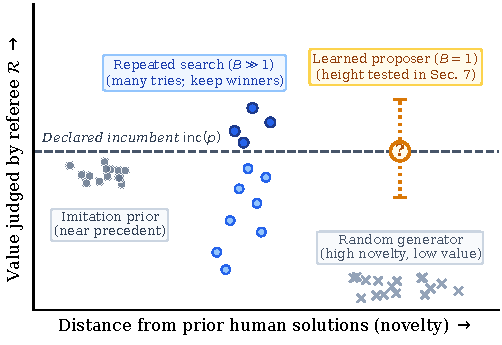
\includegraphics[width=\linewidth]{figures/fig2_novelty_judgment.pdf}
  \caption{\textbf{Novelty is free; judgment is the inventor.} Schematic. Horizontal: distance from what people have already done. Vertical: value as judged by the referee. A random generator travels far and finds little. Imitation, repeated search and a learned proposer illustrate different ways to select candidates; their positions are conceptual, not measured limits. The value of \EZ{}'s single proposal remains an empirical question for \cref{sec:results}.}
  \label{fig:novelty-judgment}
\end{figure}

Language-model studies test this distinction. In a blinded study with 104 NLP researchers, ideas from a language model were rated more original than experts' ideas ($p < 0.05$) \citep{si2024ideas}. Once 43 experts had spent over 100 hours each carrying out ideas from both pools, the generated ideas lost significantly more ground on every metric \citep{si2025gap}.

Boden had predicted the asymmetry in 1998: machines, she wrote, would find generating new ideas easier than automating their evaluation \citep{boden1998creativity}. These studies motivate a distinction between the novelty of a proposal and
its value after execution; they do not establish that judgment is the only
bottleneck in every domain.

\subsection{The four pillars}\label{sub:anatomy-pillars}

Accounts of discovery from biology, psychology, philosophy and engineering
provide a useful common vocabulary (\cref{tab:pillars}). The four-pillar
organization is our synthesis of these traditions, rather than a claim that
their theories are identical.

\textbf{Aim} fixes the problem and what counts as better. Hamming asked colleagues, ``What are the important problems of your field?'' \citep{hamming1986research}. Pólya's first step is to understand the problem \citep{polya1945solve}, and Popper argued that observation is always selective, so it presupposes a problem \citep{popper1963conjectures}.

\textbf{Variation} proposes candidates. Peirce called abduction ``the only logical operation which introduces any new idea'' \citep[CP~5.171]{peirce1934cp}. Campbell modeled creative thought as blind variation \citep{campbell1960bvsr,simonton2011bvsr}. Koestler located creative acts in bisociation, joining two unrelated frames of thought \citep{koestler1964act}. Boden named three routes to a new idea: combining familiar ideas, exploring a conceptual space and transforming it \citep{boden1998creativity}.

\textbf{Judgment} tests a candidate against something outside the mind that proposed it: the attempted refutation \citep{popper1959logic}, the experiment, peer review, and the referee of the common task framework, which scores every entry on data the competitors never see \citep{donoho2017fifty}.

\textbf{Retention} preserves what survives: inheritance for
\citet{darwin1859origin}, selective retention for
\citet{campbell1960bvsr}, the textbook for a science and the incumbent for a
game. It can store either an output or a way to propose better outputs.
Archiving a winning program does the first; using evaluation feedback to
update the generator attempts the second. This distinction connects the
four pillars to the learning question in \cref{sec:intro}.

Campbell argued that every genuine gain in knowledge needs a mechanism for introducing variation, a consistent selection process, and a mechanism for preserving and reproducing what is selected \citep[p.~381]{campbell1960bvsr}. The aim is what keeps the selection consistent, which makes it the fourth pillar.

\subsection{Taste is judgment moved upstream}\label{sub:anatomy-taste}

Skill in invention is judgment that arrives before the try. For Poincaré, creating meant not making the useless combinations: ``Invention is discernment, choice.'' The sterile combinations, he added, do not even present themselves to the inventor \citep[pp.~324--325]{poincare1910creation}.

Chess masters show the same economy: in de Groot's think-aloud studies they considered about as many moves as weaker players but found the right ones \citep{degroot1965thought}. Chase and Simon studied chunks through perception and recall tasks \citep{chase1973perception}. Much of that knowledge is tacit; experts know more than they can say \citep{polanyi1966tacit}.

AlphaGo's policy network learned to select moves from human expert games,
then refined that judgment through self-play \citep{silver2016mastering}.

Taste has a price we can state. Suppose each try beats the incumbent with a fixed, nonzero probability
$\winprob$, independently of the others. The number of tries up to and including the first win is then geometric, with mean
\begin{equation}
  \mathbb{E}[\Ntries] = \frac{1}{\winprob},
  \label{eq:taste}
\end{equation}
where $\Ntries$ counts all candidate attempts, including incomplete or
invalid outputs and failed executions. Under this fixed-probability,
independent-try model, better proposal quality
shortens the expected search.\footnote{Adaptive search and correlated
proposals need not follow \cref{eq:taste}; independence alone does not say
whether the approximation overstates or understates their cost. Empirical
attempt curves are required for those systems.}

The equation isolates the value of learning before deployment. It does not
rank random generators, pretrained models and agent systems without measuring
their proposal quality. In particular, \searchone{} fixes the number of
candidates a system may submit; it does not require the probability of a win
to approach certainty. A single-candidate system can fail, and every failure
must remain in its reported results. \Cref{sec:price} uses the same idealization
to relate evaluation cost to the cost of a verified improvement.

\begin{keyidea}
Novelty is free. Judgment is the inventor.
\end{keyidea}

\subsection{Learning from a referee}\label{sub:anatomy-history}

People learn much of their taste from the record of their field. Normal science, in Kuhn's account, solves puzzles inside a reigning paradigm \citep{kuhn1962structure}. The record also holds people in place: when a star life scientist dies prematurely, articles by outsiders to the star's collaborators flow into the field, draw on different literature and are disproportionately likely to be highly cited \citep{azoulay2019funeral}.

A model trained to predict text receives a signal about what was written,
rather than a direct score for improving an algorithm. That does not prevent
novel generalization. It motivates supplementing the historical record with
feedback from execution, so a useful departure from precedent can be rewarded.

A referee offers such an additional teacher. AlphaGo Zero learned with no human data, from the rules and the outcomes of its own games, and found strategies outside traditional Go knowledge \citep{silver2017mastering}. Its predecessor had already made such a move. As David Silver told Wired in March 2016, AlphaGo put the chance that a human would play its Move~37 against Lee Sedol at one in ten thousand, and it won that game \citep{metz2016twomoves}.

The knowledge then flowed back to people. In more than 5.8 million moves by professionals from 1950 to 2021, previously unseen moves grew more frequent once superhuman programs arrived, and came with better decisions \citep{shin2023superhuman}. These results establish the possibility in Go. Whether an analogous signal
improves algorithm invention must be measured in the innovation game.

\subsection{Where the pillars live}\label{sub:anatomy-where}

Machines do not remove the pillars; they move them (\cref{tab:where}). The most ambitious swarm design fits the same anatomy. In an October 2026 essay drawn from his book, Socher rests the Eureka Machine on ``a living map of all human knowledge'', ``a unified model of physical reality'', ``high-fidelity digital twins'' and ``fully autonomous physical laboratories'' \citep{socher2026bookbite,socher2026eureka}. On top of them, millions of AI agents critique each other's ideas. In our terms, the map is retention; the model of reality, the twins and the laboratories are faster and better judgment; and the agents supply variation and critique.

Agent search and learning from a referee are complementary. A search can
retain programs, revise its context or update its proposer; calling it a
swarm does not determine which of these it does. The comparison in
\cref{tab:where} therefore isolates a common deployment setting in which
search leaves the proposer's weights fixed. \EZ{} instead aims to use
training evaluations to improve the proposer before a new problem arrives.
Both approaches still need a reliable referee, and the cost of training
must be counted alongside any saving at deployment.

\begin{table}[t]
  \caption{\textbf{Where feedback can be retained.} The agent-search column describes
fixed-weight deployment loops, not every agent system. The \EZ{} column
states the proposed training and deployment protocol. In every column,
people still set the aim.}
  \label{tab:where}
  \centering
  \footnotesize
  \setlength{\tabcolsep}{3.5pt}
  \setlength{\extrarowheight}{2pt}% separates rows whose cells wrap
  \begin{tabular}{@{}>{\raggedright\arraybackslash}p{0.16\linewidth}>{\raggedright\arraybackslash}p{0.21\linewidth}>{\raggedright\arraybackslash}p{0.265\linewidth}>{\raggedright\arraybackslash}p{0.265\linewidth}@{}}
    \toprule
     & Human science & Agent search & \EZ{} \\
    \midrule
    Aim & The researcher chooses & A person writes the goal & Problem encoding and metric, chosen by people for now \\
    Variation & The scientist's ideas & Agents propose and critique & One candidate per test problem \\
    Judgment & Experiments, peer review & Experiments, simulators, autonomous labs & The referee, on hidden folds \\
    Retention & The literature & Logs, archives, a map of knowledge & Incumbent pool and the writer's weights \\
    \addlinespace
    Where taste lives & Years of training, in one head & Weights fixed; context can adapt & Training on referee feedback \\
    Deployment budget & Varies by problem & Multiple adaptive attempts & One candidate; success measured \\
    \bottomrule
  \end{tabular}
\end{table}

The next section traces the methods that connect these four roles.
